\documentclass[11pt]{article}
\usepackage{acl}
\usepackage{times}
\usepackage{latexsym}
\usepackage{amsmath,amssymb,amsfonts}
\usepackage{booktabs}
\usepackage{multirow}
\usepackage{graphicx}
\usepackage{url}
\usepackage{hyperref}

\title{How LoRA Fine-Tuning Changes Factual Predictions Across Transformer Layers}

\author{
  Hadas Yonat \\
  Tel Aviv University \\
  \texttt{hadasyonat@mail.tau.ac.il} \\\And
  Yuval Bukovsky \\
  Tel Aviv University \\
  \texttt{bukovsky@mail.tau.ac.il} \\\AND
  Mika Labin \\
  Tel Aviv University \\
  \texttt{mikalabin@mail.tau.ac.il} \\\And
  Gal Cohen \\
  Tel Aviv University \\
  \texttt{gc7@mail.tau.ac.il}
}

\begin{document}
\maketitle

%% ── Abstract ──────────────────────────────────────────────────────────────────
\begin{abstract}
Parameter-efficient fine-tuning methods such as LoRA can substantially improve
factual prediction accuracy, yet how these changes propagate across transformer
layers remains poorly understood.
We study \emph{where} in the forward pass LoRA writes factual knowledge by
applying logit-lens analysis and causal activation patching to Pythia-410m
fine-tuned on CounterFact.
We distinguish four conditions ordered by how much prior signal the base model
has: facts it already knows (\emph{known}), facts whose correct answer appears
in the top-5 but not top-1 with meaningful probability (\emph{latent}), real
facts with no top-5 signal (\emph{unknown}), and entirely invented facts
(\emph{synthetic}).
Causal activation patching reveals a strict ordering of encoding depth across
the three conditions where LoRA was needed: latent facts flip the base model
at layer~10 (median), unknown at layer~16, and synthetic at layer~19 out of 24.
Logit-lens trajectories provide convergent but distinct evidence: LoRA shifts
predictions \emph{earlier} for conditions with latent signal (known $-2.5$
layers, latent $-0.4$) and \emph{later} for novel facts (synthetic $+3.8$
layers).
All gains come at a steep locality cost: Kullback-Leibler (KL) divergence on 
neighboring-fact predictions over the top-50 tokens ranges from 4.9 to 5.4 nats 
across all conditions, proving LoRA induces massive representational drift 
regardless of the knowledge type.
\end{abstract}

%% ── 1. Introduction ───────────────────────────────────────────────────────────
\section{Introduction}

Low-Rank Adaptation (LoRA; \citealt{hu2022lora}) has become one of the
dominant methods for adapting large language models to new tasks.
By injecting small trainable matrices at each attention layer, LoRA achieves
competitive accuracy while updating fewer than 1\% of model parameters.
However, the improvement in final-layer predictions tells us little about
\emph{how} the model arrives at those predictions.

A natural question is whether LoRA simply amplifies an answer that was already
latent in the network, or whether it installs the answer from scratch in the
final layers.
Prior work on language adapters found that adapted predictions often shift
toward the target predominantly in the final layers
\citep{alabi2024hidden}.
Whether LoRA for factual knowledge exhibits the same late-layer pattern --- and
whether this depends on the novelty of the fact being injected --- is unknown.

We ask: \textbf{How does LoRA fine-tuning on factual knowledge affect the
evolution of predictions across transformer layers, and does this differ
along a spectrum from facts the model already knows, to facts where the
correct answer is latent but suppressed, to facts it has no signal for,
to entirely invented facts?}

To answer this, we fine-tune Pythia-410m-deduped on a stratified subset of the
CounterFact benchmark \citep{meng2022locating} and analyse the resulting model
using logit lens \citep{logitlens2020}, tuned lens \citep{belrose2023eliciting},
and causal activation patching.
We run patching at every training checkpoint (not only the final model) to
track \emph{when} causal structure emerges during training.
We supplement this with a rank ablation ($r \in \{4,8,16,32\}$) and a locality
audit on 15{,}000 neighborhood prompts using Kullback-Leibler (KL) divergence.

Our main finding is that LoRA's causal encoding depth forms a strict spectrum
for the three conditions where LoRA was required: latent (median first-flip
layer~10) $<$ unknown (16) $<$ synthetic (19) out of 24.
This ordering is stable across all 11 training checkpoints and all four ranks
tested; higher rank increases how many facts are encoded, but not where.
A particularly clean diagnostic emerges from the direction of first-layer
shifts: conditions with latent signal shift \emph{earlier} after LoRA;
conditions without shift \emph{later}. Finally, locality evaluation proves that 
LoRA is not a surgical intervention, inducing massive representational drift across all knowledge types.

%% ── 2. Related Work ──────────────────────────────────────────────────────────
\section{Related Work}

\paragraph{Parameter-efficient fine-tuning.}
\citet{hu2022lora} introduce LoRA, which freezes the pretrained weight matrix
$W$ and learns a low-rank decomposition $\Delta W = BA$ with $B \in
\mathbb{R}^{d \times r}$, $A \in \mathbb{R}^{r \times k}$.
The effective change to each layer's output is $\alpha / r \cdot BAx$, where
$\alpha$ is a fixed scaling factor.
LoRA has been applied to language modelling, instruction following, and
knowledge editing, and is the basis of most modern fine-tuning pipelines.

\paragraph{Interpreting intermediate representations.}
The logit lens \citep{logitlens2020} decodes intermediate hidden states through
the unembedding head to obtain a vocabulary distribution at each layer, enabling
inspection of how predictions evolve through the forward pass.
\citet{belrose2023eliciting} extend this with a tuned lens: a learned affine
probe per layer that predicts the final-layer output distribution more
accurately than the raw logit lens.
We use both, reporting the logit lens as the primary metric to avoid
conflating lens-specific effects with LoRA-induced changes.

\paragraph{Adapters and layer dynamics.}
\citet{alabi2024hidden} study how adapter modules and LoRA affect the
hidden-state trajectory, finding that adapted predictions shift toward the
target predominantly in the final layers for language-transfer tasks.
We test whether the same late-layer dominance appears for factual knowledge,
and whether it holds across knowledge types.

\paragraph{Factual knowledge in LLMs.}
\citet{meng2022locating} show through causal tracing that factual associations
in GPT models are primarily stored in mid-layer MLP modules.
Our activation patching adapts their methodology: we patch hidden states from
the fine-tuned model into the base model to find the earliest layer at which
the LoRA update causally determines the output.

%% ── 3. Methodology ────────────────────────────────────────────────────────────
\section{Methodology}

\subsection{Model and Dataset}
We use \textbf{Pythia-410m-deduped} \citep{biderman2023pythia}, a 24-layer
decoder-only transformer with hidden size 1{,}024.
Facts are drawn from the \textbf{CounterFact} benchmark
\citep{meng2022locating}, which provides 19{,}728 subject--relation--object
triples along with paraphrase prompts for each fact.
We retain only facts whose target answer is a single token under the model's
tokenizer, yielding 17{,}606 usable facts.

\subsection{Experimental Conditions}
We define four conditions ordered by how much prior signal the base model has
for the correct answer:
\begin{itemize}
  \item \textbf{Known (rank 1):} The base model predicts the correct answer
    as its top-1 token; 1{,}236 facts qualify (7.0\%).
  \item \textbf{Latent (rank 2--5, log-prob $> -5$):} The correct answer
    appears in the model's top-5 predictions but is not top-1, \emph{and}
    carries meaningful probability mass (answer log-prob $> -5$, i.e.\
    $p \gtrsim 0.007$; 2{,}802 facts; 15.9\%).
    The representation is present but suppressed.
    The secondary log-probability gate excludes 35 rank-2--5 facts whose
    near-zero probability signals accidental ranking rather than genuine latent
    knowledge; those facts are reassigned to the unknown pool.
  \item \textbf{Unknown (rank $>$5, or rank 2--5 with log-prob $\le -5$):}
    The correct answer has no meaningful top-5 signal at baseline
    (13{,}568 facts; 77.1\%). The model lacks the association entirely.
  \item \textbf{Synthetic:} Pseudo-entity facts created by pairing real
    relation templates (e.g.\ \emph{``\{subject\} was born in''}) with a
    randomly generated subject name and a real object from that relation.
    By construction the base model has never encountered the triple.
\end{itemize}
This four-way split tests a spectrum hypothesis: if LoRA's encoding depth is
determined by how absent the knowledge is, we predict the strict ordering
$\text{known} < \text{latent} < \text{unknown} < \text{synthetic}$
in causal first-flip layer.
We stratify-sample 500 facts per condition and 200 synthetic facts, capping
each relation at 25\%, and train for 5 epochs (535 optimizer steps).
Paraphrase prompts are held out and never used in training.

\subsection{LoRA Fine-Tuning}
We attach LoRA adapters ($r=16$, $\alpha=32$, dropout $0.05$) to the
\texttt{query\_key\_value} projections of all attention layers (1.57M trainable
parameters; 0.39\% of total).
Training uses the cross-entropy loss on the answer token only (prompt tokens
masked), AdamW with learning rate $10^{-4}$, batch size 16, and FP16 mixed precision, for 5 epochs (535
optimizer steps).
We save adapter checkpoints every 50 steps.

\subsection{Layer-wise Analysis}
For each adapter checkpoint we run the full forward pass with
\texttt{output\_hidden\_states=True} and apply the logit lens (frozen final
layer-norm $+$ unembedding head) to every intermediate hidden state at the last
token position.
We record acc@1, mean log-probability, and the first layer at which the correct
answer appears as top-1 (\emph{first-layer-of-appearance}).
The \emph{base model's} tuned lens is loaded from the AlignmentResearch hub and
kept frozen across all variants, ensuring that any change in its readout is
attributable to LoRA, not to changes in the probe.

\subsection{Causal Activation Patching}
For each fact and each layer $\ell \in \{1,\ldots,24\}$, we patch the LoRA
model's residual stream after block $\ell$ into the base model via a forward
hook, and record whether the base model's output flips to the target answer.
The \emph{first-flip layer} is the smallest $\ell$ at which the flip occurs.
A first-flip layer near 0 means the answer was already causally present
(LoRA only amplified it); a first-flip layer near 24 means the entire update
lives in the final layers.
We run patching at every training checkpoint to track how causal depth evolves
during fine-tuning.

%% ── 4. Results ────────────────────────────────────────────────────────────────
\section{Results}

\begin{table}[t]
\centering\small
\caption{Logit-lens results before and after LoRA fine-tuning (Pythia-410m-deduped, $r=16$, 535 steps).
\emph{First layer $\Delta$} = shift in mean first-appearance layer (negative = earlier).
Para.\ = held-out paraphrase prompts (never seen in training).}
\label{tab:main_results}
\resizebox{\columnwidth}{!}{%
\begin{tabular}{llccccc}
\toprule
 & & \multicolumn{2}{c}{\textbf{Acc@1}} & \multicolumn{2}{c}{\textbf{Mean log-prob}} & \textbf{First} \\
\cmidrule(lr){3-4}\cmidrule(lr){5-6}
\textbf{Condition} & \textbf{Prompts} & Base & LoRA & Base & LoRA & \textbf{layer $\Delta$} \\
\midrule
Known          & train & 0.988 & 0.988 & $-$1.62 & $-$0.09 & $-$2.5 \\
Known          & para. & 0.312 & 0.809 & $-$3.92 & $-$0.71 & $-$1.2 \\
Latent (top-5) & train & 0.002 & 0.968 & $-$3.25 & $-$0.20 & $-$0.4 \\
Latent (top-5) & para. & 0.132 & 0.745 & $-$5.03 & $-$1.00 & $-$0.7 \\
Unknown        & train & 0.000 & 0.780 & $-$7.38 & $-$0.93 & $+$1.2 \\
Unknown        & para. & 0.054 & 0.421 & $-$6.96 & $-$2.88 & $+$0.5 \\
Synthetic      & train & 0.000 & 0.590 & $-$8.84 & $-$1.79 & $+$3.8 \\
\bottomrule
\end{tabular}%
}
\end{table}

\subsection{Layer-wise Prediction Evolution}

Table~\ref{tab:main_results} shows the final-layer statistics for all four
conditions.
Figure~\ref{fig:delta_logprob} shows how LoRA's gain in answer log-probability
is distributed across the 24 transformer layers.

\begin{figure}[t]
  \centering
  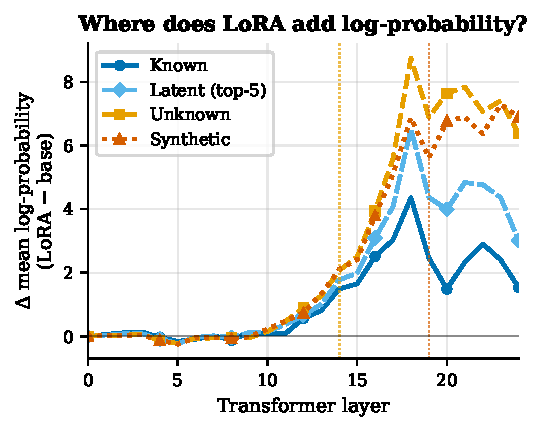
\includegraphics[width=0.85\linewidth]{figures/fig_delta_logprob.pdf}
  \caption{Mean increase in answer log-probability at each layer
  (LoRA final $-$ base, training prompts).
  Vertical dotted lines mark median causal first-flip layers for unknown
  (layer~16) and synthetic (layer~19) from patching.}
  \label{fig:delta_logprob}
\end{figure}

The four conditions show qualitatively distinct shapes that reflect their
amount of prior signal.

\textbf{Known} facts show a moderate gain that rises gradually from early layers, consistent with shallow amplification.
The first-layer-of-appearance moves 2.5 layers earlier (21.2 $\to$ 18.6) and
paraphrase accuracy jumps from 31.2\% to 80.9\%.

\textbf{Latent} facts (answer in top-5 but not top-1, and log-prob $> -5$)
show the most striking result.
Despite near-zero baseline accuracy (0.2\%), LoRA raises training accuracy to
96.8\% and held-out paraphrase accuracy to 74.5\%.
First-layer-of-appearance shifts only 0.4 layers earlier --- the lightest
structural change needed to unlock an already-present representation.
This is the clearest evidence in our results that LoRA operates as a
\emph{representation unlocker} when the knowledge exists but is suppressed.

\textbf{Unknown} facts (no meaningful top-5 signal) show a large gain
concentrated after layer~14, and the first-layer-of-appearance shifts 1.2
layers \emph{later} --- the first condition where the direction reverses.
Paraphrase accuracy reaches 42.1\%, substantially below latent (74.5\%),
reflecting the absence of prior structure to generalise from.

\textbf{Synthetic} facts show the most extreme late-layer spike pattern, with the
first-layer shift reaching $+3.8$ layers later and training accuracy of 59.0\%.

The direction of first-layer shift is itself a clean diagnostic:
conditions with latent signal (known: $-2.5$, latent: $-0.4$) shift earlier;
conditions without it (unknown: $+1.2$, synthetic: $+3.8$) shift later.
The boundary aligns exactly with the combined top-5 rank and log-probability
criterion used to define the latent condition.

\subsection{Causal Localization via Activation Patching}
\label{sec:patching}

\begin{table}[t]
\centering\small
\caption{Activation patching at the final LoRA checkpoint ($r=16$, step 535).
\emph{Flipped} = facts (out of 100) where any single-layer patch causes the
base model to output the target answer.
The known condition is excluded: the base model already predicts correctly for
those facts, so the result would reflect the selection criterion rather than
LoRA's causal footprint.}
\label{tab:patching}
\begin{tabular}{lccc}
\toprule
\textbf{Condition} & \textbf{Flipped} & \textbf{Mean first-flip layer} & \textbf{Median} \\
\midrule
Latent    & 100/100 &  9.86 & 10 \\
Unknown   &  82/100 & 15.30 & 16 \\
Synthetic &  64/100 & 18.25 & 19 \\
\bottomrule
\end{tabular}
\end{table}

\begin{figure}[t]
  \centering
  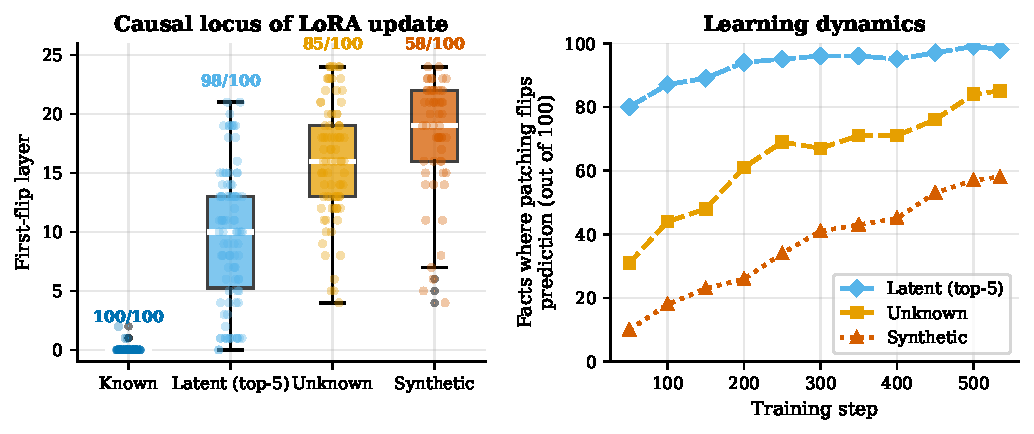
\includegraphics[width=\linewidth]{figures/fig_patching.pdf}
  \caption{\emph{Left:} Distribution of first-flip layers at the final checkpoint.
  Latent, unknown, and synthetic are cleanly separated; known is omitted from
  the causal analysis (see text).
  \emph{Right:} Count of flipped facts across 11 training checkpoints
  (known omitted; trivially 100 throughout).
  Location is stable; count grows with training.}
  \label{fig:patching}
\end{figure}

Table~\ref{tab:patching} and Figure~\ref{fig:patching} show the causal results
for the three conditions where LoRA was required to produce the correct answer.
By patching the full residual stream at each layer, we identify the earliest
point at which LoRA-modified activations are sufficient to flip the base
model's output to the target.
The strict ordering \textbf{latent} (median layer~10) $<$ \textbf{unknown}
(16) $<$ \textbf{synthetic} (19) confirms the depth spectrum.

For \textbf{latent} facts, all 100 flip at a median of layer~10, placing the
causal site in the mid-network region where \citet{meng2022locating} identified
factual associations in GPT. LoRA's intervention here is minimal: it redirects
an existing representation rather than writing a new one.
For \textbf{unknown} facts, 82/100 flip at layer~16; for \textbf{synthetic}
facts, 64/100 flip at layer~19.

The right panel of Figure~\ref{fig:patching} shows the training dynamics across
all 11 checkpoints (steps 50--535). The first-flip \emph{layer} per condition is stable throughout: latent stays near 10, unknown near 16, synthetic near 19. What grows with training is the \emph{count}. \textbf{Where LoRA encodes a fact is determined by the fact's novelty from the very first training step; training only determines how many facts reach that threshold.}

\subsection{Effect of LoRA Rank}

\begin{figure}[t]
  \centering
  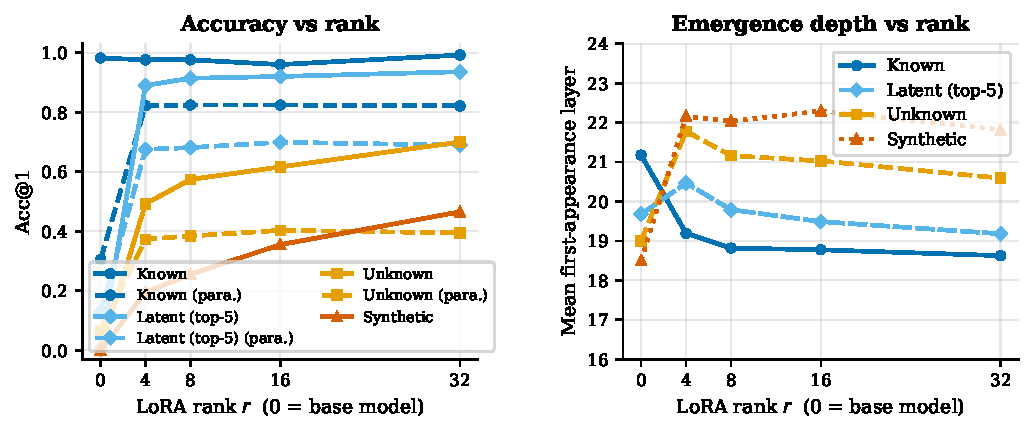
\includegraphics[width=\linewidth]{figures/fig_rank_ablation.pdf}
  \caption{\emph{Left:} Accuracy vs rank (solid = train, dashed = paraphrase).
  \emph{Right:} Mean first-appearance layer vs rank.}
  \label{fig:rank_ablation}
\end{figure}

Figure~\ref{fig:rank_ablation} confirms that rank governs capacity, not depth.
For \textbf{synthetic} facts, train accuracy scales from 25.5\% at $r=4$ to
53.5\% at $r=32$, yet the mean first-appearance layer stays near 22 throughout
($r=4$: 22.2, $r=32$: 22.1).
For \textbf{unknown} facts the pattern is similar (47.2\% to 69.2\% in accuracy), but depth drops slightly (21.4 to 20.6).
For \textbf{latent} facts, accuracy is high at all ranks (88.0\% to 94.6\%)
and depth decreases slightly with rank (20.3 to 19.0), consistent with larger
adapters making slightly more efficient use of a pre-existing representation.
\textbf{Known} facts are rank-saturated: train accuracy stays near 96--98\%
and paraphrase accuracy plateaus around $r=8$ (82.0\%), while their depth also drops (19.5 to 18.7).

The right panel makes the separation explicit: all real-world facts (known, latent, unknown) show a mild depth decrease of $\sim 0.8 - 1.2$ layers as rank increases from 4 to 32, taking advantage of the added capacity to surface answers earlier. Only synthetic facts stay strictly locked in the final layers (shifting just 0.1 layers). \textbf{Rank primarily acts as a capacity dial; the fundamental depth of extraction is still governed by the knowledge type.}

\subsection{Locality of Factual Updates}

\begin{table}[t]
\centering\small
\caption{Neighborhood locality across 5{,}000 related-fact prompts per
condition.
\emph{KL div.}\ = mean KL$(P_\text{base} \| P_\text{LoRA})$ restricted to
the top-50 tokens under the base distribution, with both distributions
renormalized over that support.
\emph{Pres.\ rate} = fraction of prompts where LoRA top-1 equals base top-1.}
\label{tab:locality}
\begin{tabular}{lccc}
\toprule
\textbf{Condition} & \textbf{KL div.} & \textbf{Pres.\ rate} & \textbf{$N$ prompts} \\
\midrule
Known          & 5.45 & 0.223 & 5{,}000 \\
Latent (top-5) & 5.32 & 0.102 & 5{,}000 \\
Unknown        & 4.92 & 0.063 & 5{,}000 \\
\bottomrule
\end{tabular}
\end{table}

Table~\ref{tab:locality} reveals an inverse relationship between distributional drift (KL) and top-1 preservation, highlighting a paradox of fine-tuning disruption. Known facts exhibit the highest top-50 KL divergence (5.45 nats) but also the highest top-1 preservation (22.3\%). Conversely, unknown facts show the lowest KL divergence (4.92 nats) but the lowest preservation (6.3\%).

This apparent paradox is explained by baseline confidence. Known facts have sharp, highly confident initial distributions; when LoRA perturbs the network, it scatters mass away from the dominant token, incurring an immense KL penalty. However, because the initial margin was so large, the top token often survives as the argmax. Unknown facts have flatter, more uniform initial distributions, so perturbations incur a smaller KL penalty but easily scramble the fragile top-1 ranking. Across all conditions, the absolute magnitude of drift (4.9--5.4 nats over just the top 50 tokens) confirms that LoRA induces massive collateral damage, regardless of depth.

%% ── 5. Discussion ─────────────────────────────────────────────────────────────
\section{Discussion}

Our results establish a consistent spectrum across two independent measurements.
Logit-lens analysis shows that LoRA's first-layer-of-appearance shifts earlier
for conditions with latent signal (known: $-2.5$ layers, latent: $-0.4$) and
later for conditions without it (unknown: $+1.2$, synthetic: $+3.8$).
Causal activation patching confirms a monotone ordering in absolute causal
depth --- but only for the three conditions where LoRA was actually needed:
\textbf{latent} (median layer~10) $<$ \textbf{unknown} (16) $<$
\textbf{synthetic} (19) out of 24.
The known condition is excluded from this causal ordering because its layer-0
result reflects the base model's pre-existing capability, not LoRA's encoding
depth (see Section~\ref{sec:patching}).

It is worth being explicit that these two measurements capture different things.
The logit-lens shift is a \emph{relative} change in the fine-tuned model's own
internal trajectory: it measures how much earlier or later the correct answer
\emph{naturally emerges} in the LoRA model versus the base model, with no
intervention.
The causal first-flip layer is an \emph{absolute} measure of causal sufficiency:
the earliest point at which LoRA-modified activations, when injected into the
\emph{base} model, are sufficient to flip its output.
The two metrics qualitatively agree --- both put conditions with prior signal
earlier and conditions without it later --- but they are not equivalent, and
their agreement should be read as corroborating convergent evidence, not as
independent confirmation of a single underlying quantity.

The latent condition is the most theoretically informative.
Latent facts yield an immense raw paraphrase generalisation gain ($\Delta = +0.613$). While this absolute delta is larger than that of known facts ($+0.497$), both conditions actually consume an identical proportion of their available accuracy headroom ($\sim 70\%$). Remarkably, latent facts achieve this elite generalisation with barely any structural change to the forward pass ($-0.4$ layers).
This combination --- large accuracy gain, maximal generalisation efficiency, and shallow causal site (layer 10) --- points to LoRA acting as a \emph{gating mechanism}: it adjusts attention weights so that a correct but suppressed representation wins the competition against the incorrect top-1 prediction.
The log-probability gate used to define the latent category (answer log-prob $> -5$) reinforces this interpretation: the 35 reclassified facts that passed the rank-2--5 criterion but carried near-zero probability are semantically closer to unknown, and excluding them sharpens the latent cluster.

Unknown-fact fine-tuning, in contrast, must operate deeper (layer 16) and
shows substantially weaker paraphrase generalisation (42.1\% vs 74.5\%),
consistent with the model constructing a narrower, less compositional
association.
Synthetic facts, with no prior structure at all, can only be installed in the
final layers (layer 19) and cannot be tested for paraphrase generalisation.

Together, these findings suggest that the late-layer dominance reported by
\citet{alabi2024hidden} for language adapters is real but incomplete:
it applies to conditions where the model has no existing signal, while LoRA
on latent or known facts operates substantially earlier.
The important variable is not task type (language transfer vs.\ factual
knowledge) but the degree to which the knowledge already exists in the network.

A limitation is that all four conditions are trained jointly, meaning condition interactions cannot be disentangled without separate runs. Additionally, because synthetic subjects are generated pseudo-words, they are likely subjected to irregular subword fragmentation by the BPE tokenizer. This may induce out-of-distribution attention patterns compared to real entities, partially contributing to their delayed, late-layer extraction.

%% ── 6. Conclusion ─────────────────────────────────────────────────────────────
\section{Conclusion}

We have shown that LoRA fine-tuning for factual knowledge produces a consistent
encoding-depth spectrum determined by prior knowledge, visible through both
logit-lens trajectories and causal activation patching.
The causal ordering spans the three conditions where LoRA was needed: latent
facts (answer in top-5 with log-prob $> -5$) are encoded at median layer~10,
unknown facts at layer~16, and synthetic facts at layer~19 out of 24.
The known condition is a control: because the base model already answers
correctly, its layer-0 patching result reflects the inclusion criterion, not
LoRA's causal footprint.
The depth ordering is stable across all 11 training checkpoints and all four
ranks tested ($r \in \{4,8,16,32\}$): training increases how many facts are
encoded, rank increases how many can be encoded, but neither changes where.

The latent condition is the practical takeaway: LoRA is most efficient when
the correct answer is already in the model's top-5 predictions \emph{with
meaningful probability} (log-prob $> -5$), delivering 96.8\% train accuracy
and 74.5\% paraphrase generalisation --- performing as well as known facts ---
from the smallest structural change.
All conditions degrade locality severely: top-1 preservation rates range from
22.3\% (known) down to 6.3\% (unknown). We find that LoRA induces immense representational drift across all conditions, though sharp initial distributions (known facts) are paradoxically more robust to losing their argmax ranking despite incurring higher KL divergence penalties.

Practitioners who need high locality should prefer fine-tuning on facts where
the model already has latent signal (top-5 and log-prob $> -5$ at baseline),
monitor neighborhood KL-divergence during training as an early warning signal,
and treat synthetic-entity injection as a last resort given its combination of
low generalisation and deep structural cost.

%% ── AI Disclosure ─────────────────────────────────────────────────────────────
\section*{AI Disclosure and Reflection}

We used Claude (Anthropic) and GitHub Copilot to assist with implementation
debugging, data-pipeline design, and manuscript editing.
The experimental design, hypotheses, analysis, and conclusions are our own.
All reported numbers were produced by running our code on Google Colab A100
hardware and verified manually against the raw output logs.

%% ── References ────────────────────────────────────────────────────────────────
\bibliography{references}
\bibliographystyle{acl_natbib}

\end{document}